\documentclass[tikz,border=4pt]{standalone}

\usepackage{tikz}
\usetikzlibrary{calc}

\begin{document}

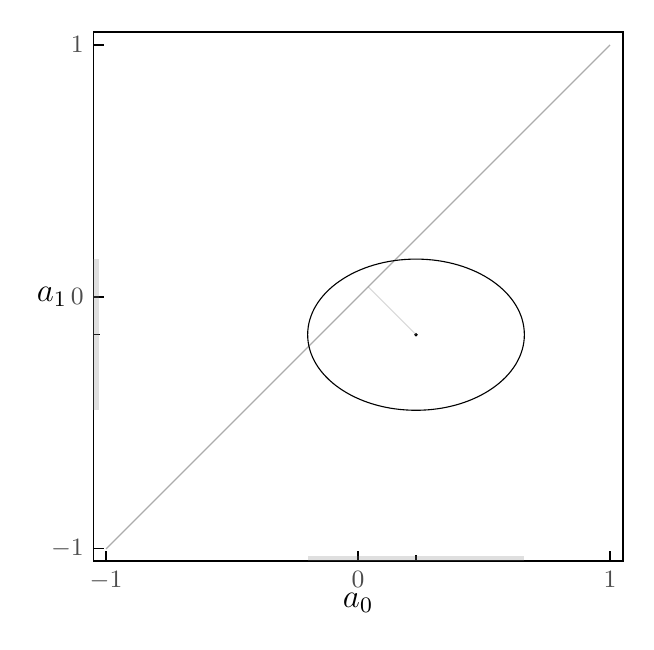
\begin{tikzpicture}[
    x=3.2cm,
    y=3.2cm,
    tick/.style={black, line width=0.45pt},
    frame/.style={black, line width=0.7pt},
    agreement/.style={gray!65, line width=0.45pt},
    axislabel/.style={font=\large},
    ticklabel/.style={font=\small, text=black!70}
]

% -------------------------------------------------------------------------
% Limits
% -------------------------------------------------------------------------
\def\xmin{-1.05}
\def\xmax{ 1.05}
\def\ymin{-1.05}
\def\ymax{ 1.05}

\def\ticklen{0.02}

% -------------------------------------------------------------------------
% Agreement line
% -------------------------------------------------------------------------
\draw[ agreement ]
    (-1,-1) -- (1,1);

% -------------------------------------------------------------------------
% Frame
% -------------------------------------------------------------------------
\draw[ frame ]
    (\xmin,\ymin) rectangle (\xmax,\ymax);

% -------------------------------------------------------------------------
% Tick marks: x-axis positions
% -------------------------------------------------------------------------
\foreach \x in {-1,0,1}{
    \draw[ tick ]
        (\x,\ymin) -- ++(0, 2 * \ticklen);
}

% -------------------------------------------------------------------------
% Tick marks: y-axis positions
% -------------------------------------------------------------------------
\foreach \y in {-1,0,1}{
    \draw[ tick ]
        ( \xmin,\y ) -- ++( 2 * \ticklen,0);
}

% -------------------------------------------------------------------------
% Tick labels
% -------------------------------------------------------------------------

\node[ ticklabel, below ] at (-1,\ymin) {$-1$};
\node[ ticklabel, below ] at ( 0,\ymin) {$0$};
\node[ ticklabel, below ] at ( 1,\ymin) {$1$};

\node[ ticklabel, left ] at (\xmin,-1) {$-1$};
\node[ ticklabel, left ] at (\xmin, 0) {$0$};
\node[ ticklabel, left ] at (\xmin, 1) {$1$};

% -------------------------------------------------------------------------
% Axis labels
% -------------------------------------------------------------------------

\node[ axislabel, below = 8pt ] at (0,\ymin) {$a_0$};
\node[ axislabel, left = 6pt ] at (\xmin,0) {$a_1$};

% -------------------------------------------------------------------------
% Ellipse 
% -------------------------------------------------------------------------

% draw the ellipse: center at (mu0, mu1), radii (sigma0, sigma1)
\coordinate (ellipse-center) at (0.23,-0.15);

\def\sigmaZero{0.43}
\def\sigmaOne{0.30}

\draw (ellipse-center)
    ellipse [ x radius=0.43, y radius=0.30 ];
% Small ticks marking the ellipse-center coordinates
\draw[ thin ] (ellipse-center |- 0,\ymin) -- ++(0,0.025);
\draw[ thin ] (ellipse-center -| \xmin,0) -- ++(0.025,0);
% mark ellip[se origin]
\fill (ellipse-center) circle (0.0075);

% minimum distance to agreement line
% x = ( mu0 + mu1 ) / 2; y = x
\draw[ thin, gray, opacity=0.3 ] (ellipse-center) -- (0.04,0.04);

% shade one standard deviation
% Standard-deviation smear on the a_0 axis
\path[fill=gray, opacity=0.25]
    ($(ellipse-center |- 0,\ymin) + (-\sigmaZero,0)$)
    rectangle
    ($(ellipse-center |- 0,\ymin) + (\sigmaZero,\ticklen)$);

% Standard-deviation smear on the a_1 axis
\path[fill=gray, opacity=0.25]
    ($(ellipse-center -| \xmin,0) + (0,-\sigmaOne)$)
    rectangle
    ($(ellipse-center -| \xmin,0) + (\ticklen,\sigmaOne)$);
    
\end{tikzpicture}

\end{document}
